\chapter{光合作用与自养}\label{ch:b1:photosynthesis}

兔子、橡树、读者和这一页中的每一克碳，
原本都是空气中的二氧化碳，经
由一片叶子——或藻类、蓝细菌——借助阳光的能量
\omterm{def:b1:photosynthesis:fixation}{固定}为糖。该反应中，六个 $\mathrm{CO_2}$ 与六个水生成一个
葡萄糖和六个氧气，吸能 \qty{2870}{kJ/mol}；叶片
借光裂解水，将电子储存于 NADPH，
能量储存于 \omterm{def:b1:water-small-molecules:atp}{ATP}，并在合成糖的循环中消耗二者。本章
描述\omterm{def:b1:photosynthesis:chloroplast}{叶绿体}、色素，以及产生 \omterm{def:b1:water-small-molecules:atp}{ATP} 和 NADPH 的\omterm{prop:b1:photosynthesis:lightreactions}{光反应}，
\omterm{def:b1:photosynthesis:fixation}{固定}碳的\omterm{def:b1:photosynthesis:fixation}{卡尔文循环}，
称为光呼吸的漏损，以及堵住它的两种方式，
并阐述\omterm{def:b1:photosynthesis:autotrophy}{自养}的一般含义。

\section{叶绿体及其色素}

\begin{definition}[叶绿体]\label{def:b1:photosynthesis:chloroplast}
\emph{叶绿体}\index{叶绿体}是一种透镜状的\omterm{def:b1:eukaryotic-cell:organelle}{细胞器}，
长 \qtyrange{3}{10}{\micro m}，由两层包膜包被，其
内部即\emph{基质}\index{基质}，含碳\omterm{def:b1:photosynthesis:fixation}{固定}的酶、
\omterm{def:b1:carbohydrates:polysaccharide}{淀粉}粒、核糖体和一条环状 \omterm{def:b1:nucleic-acids:chain}{DNA}；基质内
另有第三套膜系统，即\emph{类囊体}\index{类囊体}，
呈扁平囊状，堆叠成\emph{基粒}，并以
鳃小片相连，包围一个连续的\emph{类囊\omterm{def:b1:body-plans-tissues:layers}{体腔}}。\omterm{prop:b1:photosynthesis:lightreactions}{光
反应}在类囊体膜上进行，碳\omterm{def:b1:photosynthesis:fixation}{固定}在
基质中进行。一个叶片\omterm{def:b1:cell-unit-of-life:cell}{细胞}含 \qtyrange{20}{100}{} 个叶绿体；每
平方毫米叶片约有五十万个。
\end{definition}

\begin{omfigure}
\begin{tikzpicture}
  \node[anchor=south west, inner sep=0] (img) at (0,0)
    {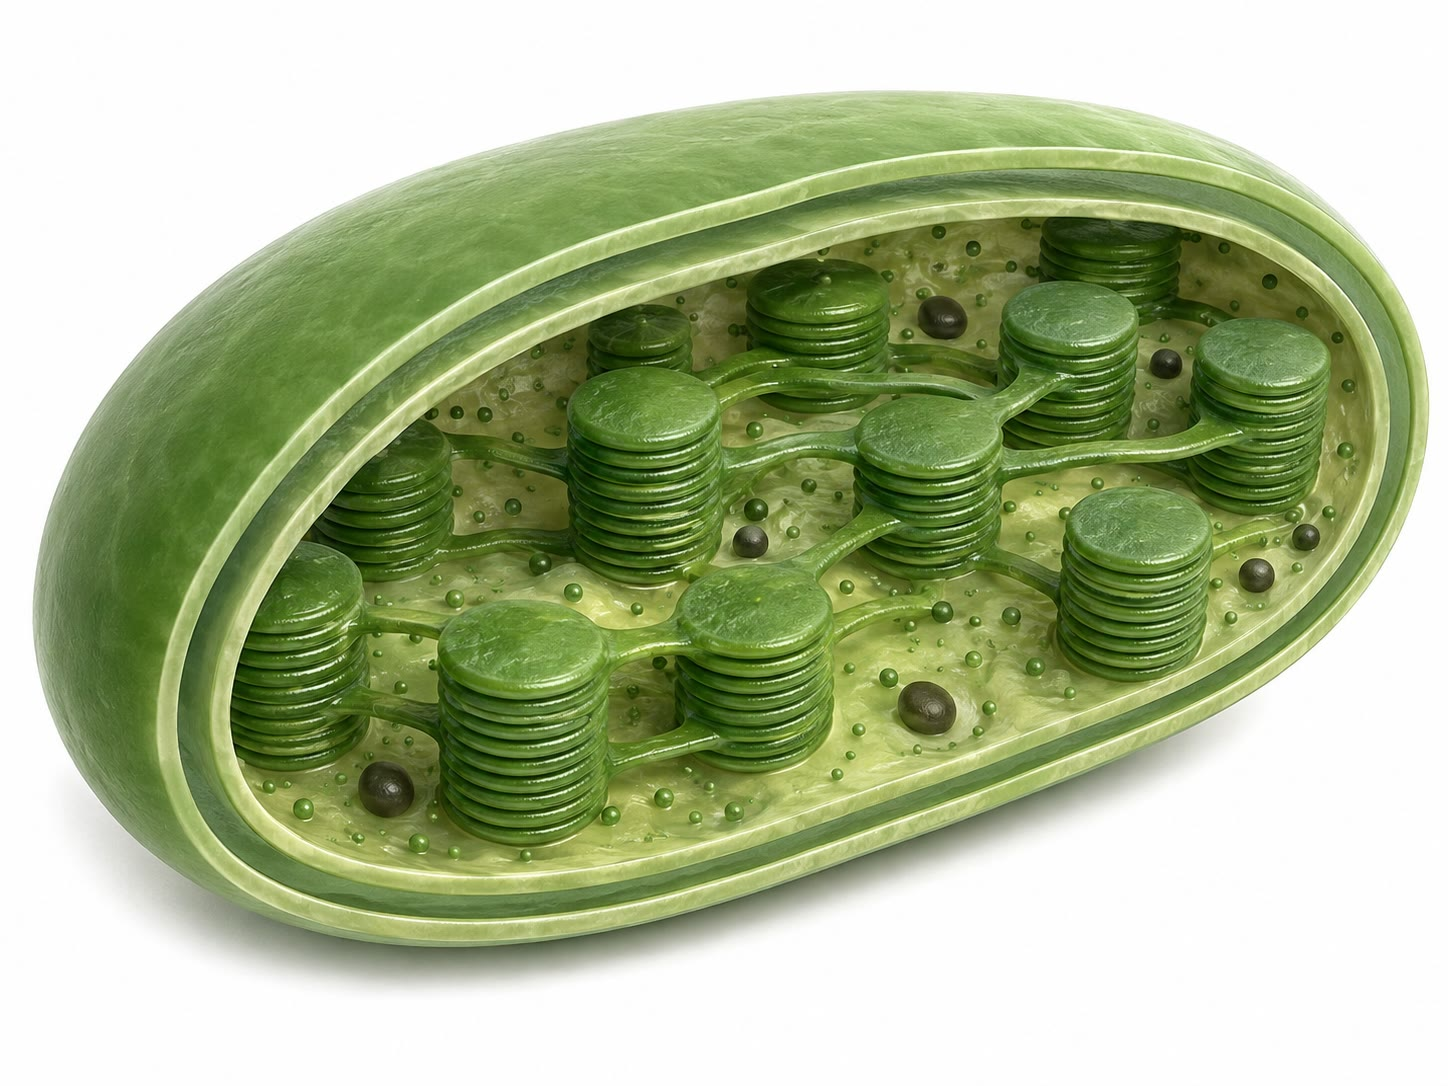
\includegraphics[width=0.56\linewidth]{images/book3/ai/fig-chloroplast-cutaway.jpg}};
  \begin{scope}[x={(img.south east)}, y={(img.north west)},
      every node/.style={font=\small}]
    \draw[omDef, thick] (0.12,0.50) -- (-0.03,0.66) node[left, align=right] {两层 \\ 包膜};
    \draw[omDef, thick] (0.48,0.60) -- (0.48,1.08) node[above] {基粒：类囊体堆叠};
    \draw[omDef, thick] (0.62,0.52) -- (1.03,0.62) node[right] {基质鳃小片};
    \draw[omDef, thick] (0.35,0.24) -- (-0.03,0.16) node[left] {基质};
    \draw[omDef, thick] (0.86,0.50) -- (1.03,0.40) node[right] {淀粉粒};
  \end{scope}
\end{tikzpicture}

{\small 剖开的\omterm{def:b1:photosynthesis:chloroplast}{叶绿体}。两层包膜包围
\omterm{def:b1:photosynthesis:chloroplast}{基质}；内部是\omterm{def:b1:photosynthesis:chloroplast}{类囊体}堆叠形成的基粒，由鳃小片相连，
并包围一个连续的\omterm{def:b1:photosynthesis:chloroplast}{类囊体}腔。光在\omterm{def:b1:photosynthesis:chloroplast}{类囊体}膜上被捕获，
糖则在\omterm{def:b1:photosynthesis:chloroplast}{基质}中合成。}
\end{omfigure}

\begin{definition}[光合色素]\label{def:b1:photosynthesis:pigments}
\emph{叶绿素}\index{叶绿素} $a$ 和 $b$ 是卟啉环，
围绕一个镁原子，带有一条长的疏水尾巴，将其
锚定于\omterm{def:b1:photosynthesis:chloroplast}{类囊体}膜中；它们吸收蓝光（\qtyrange{430}{450}{nm}）和
红光（\qtyrange{640}{680}{nm}），并反射绿光。
\emph{类胡萝卜素}\index{类胡萝卜素}（\omterm{def:b1:lipids:steroids}{类异戊二烯}，见\cref{ch:b1:lipids}）
吸收蓝绿光，并将能量传给叶绿素，
并以淬灭多余激发的方式保护它。数百个色素
分子结合于\omterm{def:b1:proteins:peptide}{蛋白质}上，组成\emph{天线}（捕光
复合体），将每个被吸收光子的能量汇集到一对特殊的
叶绿素 $a$ 分子上，即\emph{反应中心}，能量在此
被转化为化学能。
\end{definition}

\begin{omfigure}
\begin{tikzpicture}
\begin{axis}[
  width=0.88\linewidth, height=6.2cm,
  axis x line=bottom, axis y line=left,
  xmin=400, xmax=720, ymin=0, ymax=1.1,
  xlabel={波长（\unit{nm}）}, ylabel={吸收或速率（相对值）},
  xlabel style={font=\small, at={(axis description cs:0.5,-0.12)}, anchor=north},
  ylabel style={font=\small},
  tick label style={font=\small}, xtick={400,450,500,550,600,650,700}, ytick={0,0.5,1},
  legend style={font=\small, at={(0.5,0.98)}, anchor=north, draw=none},
  clip=false,
]
\addplot[very thick, omDef, domain=400:720, samples=160] {exp(-((x-430)/18)^2) + 0.85*exp(-((x-662)/14)^2) + 0.05};
\addlegendentry{叶绿素 $a$ 的吸收}
\addplot[very thick, omExo, domain=400:720, samples=160] {0.7*exp(-((x-455)/20)^2) + 0.5*exp(-((x-645)/14)^2) + 0.05};
\addlegendentry{叶绿素 $b$ 的吸收}
\addplot[very thick, omProp, domain=400:720, samples=160] {0.75*exp(-((x-470)/25)^2) + 0.05};
\addlegendentry{类胡萝卜素的吸收}
\addplot[very thick, dashed, omThm, domain=400:720, samples=160] {0.9*exp(-((x-440)/30)^2) + 0.35*exp(-((x-520)/50)^2) + 0.85*exp(-((x-660)/22)^2) + 0.1};
\addlegendentry{作用光谱：$\mathrm{O_2}$ 释放速率}
\end{axis}
\end{tikzpicture}

{\small 三类色素的吸收光谱，以及光合作用的
作用光谱（各波长下氧气的释放速率）。它
随\omterm{def:b1:photosynthesis:pigments}{叶绿素}变化，蓝绿光区则由\omterm{def:b1:photosynthesis:pigments}{类胡萝卜素}补足，
凡能吸收光的色素
都有贡献。}
\end{omfigure}

\begin{proposition}[作用光谱随色素而变]\label{prop:b1:photosynthesis:engelmann}
光合作用由色素吸收的光驱动：
在红光与蓝光下最快，在绿光下最慢。
\end{proposition}
\begin{proof}[证据]
恩格尔曼（1882 年）在显微镜下，将一条丝状藻横置于投射的光谱中，
并加入趋氧细菌：它们聚集
在红光与蓝光照射处，而不在绿光处（回顾
高中分册）。用氧电极测量，各波长下的速率
给出上文所示的作用光谱，它与
\omterm{def:b1:photosynthesis:pigments}{叶绿素}的吸收一致；蓝绿光区多出的部分
来自\omterm{def:b1:photosynthesis:pigments}{类胡萝卜素}的贡献，表明它们会将能量传递下去。
\end{proof}

\section{光反应}

\begin{proposition}[光反应的作用]\label{prop:b1:photosynthesis:lightreactions}
\index{光反应}
在\omterm{def:b1:photosynthesis:chloroplast}{类囊体}膜上，光能被用来将电子从
水转移到 $\mathrm{NADP^+}$——“上坡”进行，逆着
\qty{1.1}{V} 的氧化还原电位差——并将质子泵入\omterm{def:b1:photosynthesis:chloroplast}{类囊体}腔：
\[
2\,\mathrm{H_2O} + 2\,\mathrm{NADP^+} + 3\,\mathrm{ADP} + 3\,\mathrm{P_i}
\xrightarrow{\ 8\ \text{光子}\ }
\mathrm{O_2} + 2\,\mathrm{NADPH} + 2\,\mathrm{H^+} + 3\,\mathrm{ATP} .
\]
释放的氧气来自水，而非二氧化碳；
NADPH 携带还原力，\omterm{def:b1:water-small-molecules:atp}{ATP} 携带能量，
供\omterm{def:b1:photosynthesis:fixation}{卡尔文循环}消耗。
\end{proposition}
\begin{proof}[证据]
希尔（1937 年）证明，离体\omterm{def:b1:photosynthesis:chloroplast}{叶绿体}在光照下
在缺乏 $\mathrm{CO_2}$ 时仍能释放氧气，前提是存在人工电子受体：
水的裂解可与碳\omterm{def:b1:photosynthesis:fixation}{固定}分离。
鲁宾与卡门（1941 年）用重氧标记的水喂养藻类，
发现标记出现在释放的 $\mathrm{O_2}$ 中，
而标记在 $\mathrm{CO_2}$ 中时则不然。爱默生（1957 年）发现，
\qty{700}{nm} 的红光单独几乎无效，而 \qty{680}{nm} 的光
两者合用时的速率超过各自单独速率之和：两个
具有不同色素的\omterm{def:b1:photosynthesis:zscheme}{光系统}必须串联工作。
\end{proof}

\begin{definition}[光系统与 Z 方案]\label{def:b1:photosynthesis:zscheme}
\index{光系统}\index{Z 方案}
\omterm{def:b1:photosynthesis:chloroplast}{类囊体}膜上有两个\emph{光系统}。在
\emph{光系统 II}（PSII，反应中心 P680）中，被吸收的光子
将特殊对中的一个电子激发至高能态；该电子
离开后，被氧化的 P680，是生物界最强的氧化剂，
从水中夺取一个电子：锰簇将两个水
分子裂解为 $\mathrm{O_2}$、四个质子（释放入\omterm{def:b1:photosynthesis:chloroplast}{类囊体}腔）
和四个电子，每次只需一个光子。电子沿着
\emph{电子传递链}——\omterm{def:b1:eukaryotic-cell:plastid}{质体}醌、
\emph{\omterm{def:b1:cell-unit-of-life:cell}{细胞}色素 $b_6f$ 复合体}、\omterm{def:b1:eukaryotic-cell:plastid}{质体}蓝素——释放的能量
将质子泵入\omterm{def:b1:photosynthesis:chloroplast}{类囊体}腔。在\emph{光系统 I}（PSI，
P700）中，第二个光子再次将其提升，使电位足够低，以便
将铁氧还蛋白，继而将 $\mathrm{NADP^+}$ 还原为 NADPH。以氧化还原电位标度作图，
路径呈 Z 形：两次由光驱动的上升，两次
由化学过程驱动的下降。
\end{definition}

\begin{omfigure}
\begin{tikzpicture}[font=\footnotesize, >=Stealth, line cap=round,
  st/.style={draw, thick, rounded corners=2pt, inner sep=2pt}]
  % redox potential axis (vertical, more negative up)
  \draw[->, thick] (0,0) -- (0,6.4) node[above, font=\small] {氧化还原电位 $E'_0$（V）};
  \foreach \y/\l in {0.4/{$+1.0$}, 1.9/{$+0.5$}, 3.4/{$0$}, 4.9/{$-0.5$}, 6.0/{$-0.9$}} { \draw (-0.1,\y) -- (0.1,\y) node[left, xshift=-4pt] {\l}; }
  % PSII
  \node[st, fill=omDef!15] (h2o) at (1.7,1.0) {$\mathrm{H_2O}$};
  \node[st, fill=omDef!25] (p680) at (2.9,0.35) {P680};
  \node[st, fill=omDef!25] (p680s) at (2.9,5.7) {P680*};
  \draw[->, thick] (h2o) -- (p680);
  \node[anchor=west, font=\scriptsize] at (3.5,0.35) {$\to \mathrm{O_2} + 4\,\mathrm{H^+}$ 进入类囊体腔};
  \draw[->, very thick, omProp] (p680) -- (p680s) node[pos=0.45, right, align=left] {光子 \\ (\qty{680}{nm})};
  % chain
  \node[st, fill=omThm!15] (pq) at (4.2,4.4) {PQ};
  \node[st, fill=omThm!15] (b6f) at (5.4,3.6) {细胞色素 $b_6f$};
  \node[st, fill=omThm!15] (pc) at (6.5,2.8) {PC};
  \draw[->, thick] (p680s) -- (pq); \draw[->, thick] (pq) -- (b6f); \draw[->, thick] (b6f) -- (pc);
  \node[anchor=south west, align=left, font=\scriptsize, omThm] at (4.75,4.15) {$\mathrm{H^+}$ 泵入 \\ 类囊体腔};
  % PSI
  \node[st, fill=omExo!25] (p700) at (7.7,2.3) {P700};
  \node[st, fill=omExo!25] (p700s) at (7.7,6.0) {P700*};
  \draw[->, thick] (pc) -- (p700);
  \draw[->, very thick, omProp] (p700) -- (p700s) node[pos=0.45, right, align=left] {光子 \\ (\qty{700}{nm})};
  \node[st, fill=omThm!15] (fd) at (9.1,5.2) {Fd};
  \node[st, fill=omExo!15] (nadp) at (10.5,4.6) {NADPH};
  \draw[->, thick] (p700s) -- (fd); \draw[->, thick] (fd) -- (nadp);
  \node[anchor=north, font=\scriptsize] at (10.5,4.3) {$E'_0 = \qty{-0.32}{V}$};
  % cyclic flow
  \draw[->, thick, dashed, gray] (fd) .. controls (7.2,5.5) and (4.4,5.5) .. (pq.north);
  \node[gray, font=\scriptsize, anchor=south] at (5.6,5.45) {循环式电子流（仅产生 ATP）};
\end{tikzpicture}

{\small Z 方案。由 P680 从水中夺取的电子经
光子提升，沿泵送质子的链下降，再被 P700 提升，
最终交给 NADPH。纵轴为氧化还原电位，越负越
靠上：光负责上升，化学过程负责下降。}
\end{omfigure}

\begin{theorem}[ATP 的化学渗透合成]\label{thm:b1:photosynthesis:chemiosmosis}
\index{化学渗透}\index{ATP 合酶}
水裂解释放并由\omterm{def:b1:cell-unit-of-life:cell}{细胞}色素
$b_6f$ 复合体泵入的质子在\omterm{def:b1:photosynthesis:chloroplast}{类囊体}腔中积累，光照下该腔
\omterm{def:b1:water-small-molecules:ph}{pH} 降至 5，而\omterm{def:b1:photosynthesis:chloroplast}{基质}升至 \omterm{def:b1:water-small-molecules:ph}{pH} 8：相差三个
单位，质子动力势约为 \qty{0.18}{V}，相当于
每摩尔质子 \qty{17}{kJ}。\emph{\omterm{def:b1:water-small-molecules:atp}{ATP} 合酶}是一种
横跨\omterm{def:b1:photosynthesis:chloroplast}{类囊体}膜的旋转马达，使质子回流
进入\omterm{def:b1:photosynthesis:chloroplast}{基质}，并利用该能量使 ADP 磷酸化：每
生成一个 \omterm{def:b1:water-small-molecules:atp}{ATP} 约需 \qty{4}{H^+}。电子传递与 \omterm{def:b1:water-small-molecules:atp}{ATP} 合成
仅通过这一梯度相互偶联（米切尔化学渗透学说，1961 年）。
\end{theorem}
\begin{proof}[证据]
亚根多夫（1966 年）将\omterm{def:b1:photosynthesis:chloroplast}{类囊体}在黑暗中浸入酸浴（\omterm{def:b1:water-small-molecules:ph}{pH} 4）中，
使其\omterm{def:b1:photosynthesis:chloroplast}{类囊体}腔变酸，然后突然转入 \omterm{def:b1:water-small-molecules:ph}{pH} 8 的
含 ADP 与磷酸的溶液中：\omterm{def:b1:water-small-molecules:atp}{ATP} 在黑暗中生成，所需能量完全
来自梯度。解偶联剂——即能携带质子穿过膜的脂溶性弱酸——
会使 \omterm{def:b1:water-small-molecules:atp}{ATP} 合成完全停止，而电子传递
与放氧照常进行，甚至加快。分离出的 \omterm{def:b1:water-small-molecules:atp}{ATP} 合酶
经重组到人工囊泡中后，当施加 \omterm{def:b1:water-small-molecules:ph}{pH} 梯度时即合成 \omterm{def:b1:water-small-molecules:atp}{ATP}，
而在无梯度时则水解 \omterm{def:b1:water-small-molecules:atp}{ATP} 以泵送质子。该
酶的旋转此后已被直接观察到，
逐个分子地在显微镜下观测。
\end{proof}

\begin{example}[循环式与非循环式电子流]\label{ex:b1:photosynthesis:cyclic}
线性路径从水到 NADPH，每 $\mathrm{O_2}$ 产生两个
NADPH 和约三个 \omterm{def:b1:water-small-molecules:atp}{ATP}；\omterm{def:b1:photosynthesis:fixation}{卡尔文循环}所需的 \omterm{def:b1:water-small-molecules:atp}{ATP} 与 NADPH 之比恰为三比二，
\omterm{def:b1:photosynthesis:chloroplast}{叶绿体}的其他活动还需要更多 \omterm{def:b1:water-small-molecules:atp}{ATP}。
当 \omterm{def:b1:water-small-molecules:atp}{ATP} 不足时，来自铁氧还蛋白的电子回流至\omterm{def:b1:eukaryotic-cell:plastid}{质体}醌，
而不流向 $\mathrm{NADP^+}$（\emph{循环式
光磷酸化}）：仅由\omterm{def:b1:photosynthesis:zscheme}{光系统} I 完成，泵送质子并合成 \omterm{def:b1:water-small-molecules:atp}{ATP}，
不放氧，也不产生 NADPH。两种模式依需求取得平衡。
\end{example}

\section{卡尔文循环}

\begin{definition}[碳固定]\label{def:b1:photosynthesis:fixation}
\index{卡尔文循环}\index{RuBisCO}
\omterm{def:b1:photosynthesis:chloroplast}{基质}中的\emph{卡尔文循环}将 $\mathrm{CO_2}$ 固定为糖，
分三个阶段。\emph{固定}：\emph{RuBisCO}（核酮糖-1,5-二磷酸
羧化酶/加氧酶）将 $\mathrm{CO_2}$ 加到
核酮糖-1,5-二磷酸（RuBP，五碳）上，生成的六碳产物
随即裂解为两分子 3-磷酸甘油酸
（3-PGA，三碳）。\emph{还原}：每分子 3-PGA 被 \omterm{def:b1:water-small-molecules:atp}{ATP} 磷酸化，
并经 NADPH 还原为 3-磷酸甘油醛（G3P），即
第一个糖。\emph{再生}：每六分子 G3P 中有五分子
在消耗 \omterm{def:b1:water-small-molecules:atp}{ATP} 的情况下重排，再生为三分子 RuBP，其余一分子 G3P 离开循环，
作为净产物。一分子 G3P（三碳）的化学计量关系为
\[
3\,\mathrm{CO_2} + 9\,\mathrm{ATP} + 6\,\mathrm{NADPH} + 6\,\mathrm{H^+}
\to \text{G3P} + 9\,\mathrm{ADP} + 8\,\mathrm{P_i} + 6\,\mathrm{NADP^+} ;
\]
两分子 G3P 合成一分子葡萄糖，每分子葡萄糖需 \qty{18}{} \omterm{def:b1:water-small-molecules:atp}{ATP} 和 \qty{12}{NADPH}。
\end{definition}

\begin{omfigure}
\begin{tikzpicture}[font=\footnotesize, >=Stealth, line cap=round,
  box/.style={draw, thick, rounded corners=3pt, minimum height=8mm, align=center, fill=white}]
  \node[box, fill=omDef!15] (rubp) at (0,2.6) {3 分子核酮糖-1,5-二磷酸 \\ ($3\times$ C5)};
  \node[box, fill=omDef!15] (pga) at (5.0,2.6) {6 个 3-PGA\\ ($6\times$ C3)};
  \node[box, fill=omDef!15] (g3p) at (5.0,-0.4) {6 个 G3P\\ ($6\times$ C3)};
  \node[box, fill=omExo!20] (out) at (9.2,-0.4) {1 个 G3P 移出 \\ （净增 3 个 C）};
  \draw[->, very thick, omThm] (rubp) -- (pga) node[midway, above, align=center] {固定（RuBisCO）\\ $+\,3\,\mathrm{CO_2}$};
  \draw[->, very thick, omThm] (pga) -- (g3p) node[midway, right, align=left] {还原 \\ $6\,\mathrm{ATP}$，$6\,\mathrm{NADPH}$};
  \draw[->, very thick, omThm] (g3p) -- (out);
  \draw[->, very thick, omThm] (g3p) -| (rubp);
  \node[anchor=north, align=center, omThm] at (2.4,-0.95) {再生：5 个 G3P $\to$ 3 分子核酮糖-1,5-二磷酸 \\ $3\,\mathrm{ATP}$};
  \node[anchor=north, align=center, gray] at (4.6,-1.7) {每轮（三个 $\mathrm{CO_2}$）：9 个 ATP、6 个 NADPH，净得一个 G3P\\ 两轮：一个葡萄糖，18 个 ATP、12 个 NADPH};
\end{tikzpicture}

{\small 三个 $\mathrm{CO_2}$ 分子的\omterm{def:b1:photosynthesis:fixation}{卡尔文循环}：三分子
核酮糖-1,5-二磷酸被\omterm{def:b1:photosynthesis:fixation}{固定}为六分子 3-PGA，还原为六分子 G3P，其中一分子离开，
五分子再生为三分子核酮糖-1,5-二磷酸。碳在每一步都守恒
($15 + 3 = 18 = 3 + 15$).}
\end{omfigure}

\begin{proposition}[卡尔文的证据]\label{prop:b1:photosynthesis:calvin}
$\mathrm{CO_2}$ \omterm{def:b1:photosynthesis:fixation}{固定}后的第一个稳定产物是 3-磷酸甘油酸，
其受体为核酮糖-1,5-二磷酸。
\end{proposition}
\begin{proof}[证据]
卡尔文与本森（1948--1954）用光照射扁平烧瓶中的藻类（即
“棒棒糖”），注入 $\mathrm{^{14}CO_2}$，并在数秒后将样品投入沸腾的
酒精中杀死；二维纸色谱法
与放射自显影显示了标记所在位置。五秒后
几乎全部标记都在 3-PGA 中；较长时间的照射使标记扩散经过
糖磷酸，随后进入蔗糖和\omterm{def:b1:carbohydrates:polysaccharide}{淀粉}。当
$\mathrm{CO_2}$ 突然被撤去时，RuBP 积累，3-PGA 减少；
光照关闭时，3-PGA 积累，RuBP 减少——由此可知，
RuBP 是被\omterm{def:b1:photosynthesis:fixation}{固定}消耗的受体，3-PGA 则是
被\omterm{prop:b1:photosynthesis:lightreactions}{光反应}的 \omterm{def:b1:water-small-molecules:atp}{ATP} 与 NADPH 消耗的产物。
\end{proof}

\begin{omfigure}
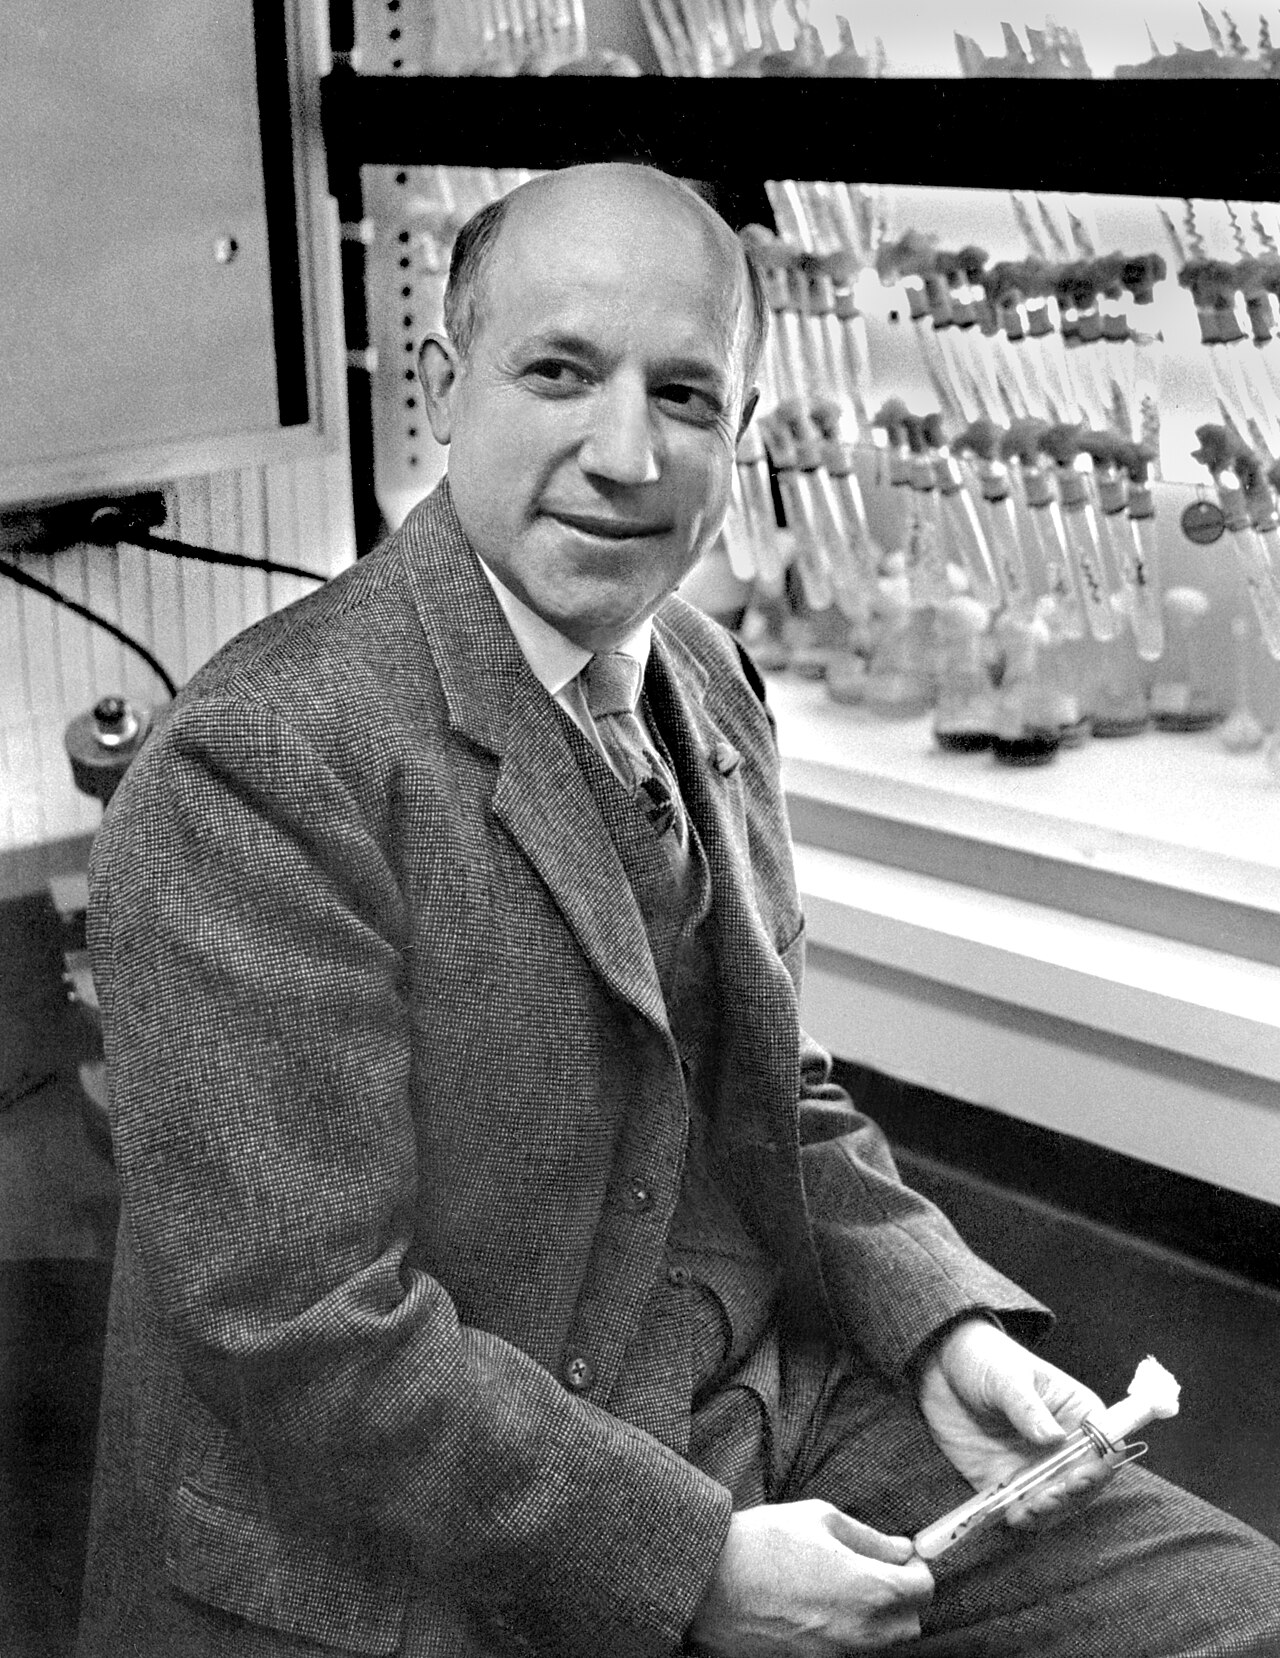
\includegraphics[width=0.26\linewidth]{images/book3/calvin.jpg}

{\small 卡尔文（1911--1997），与本森一道追踪
碳从 $\mathrm{CO_2}$ 到糖的途径，使用放射性碳与纸
色谱法。照片：Lawrence Berkeley Laboratory，公有
领域。}
\end{omfigure}

\begin{omfigure}
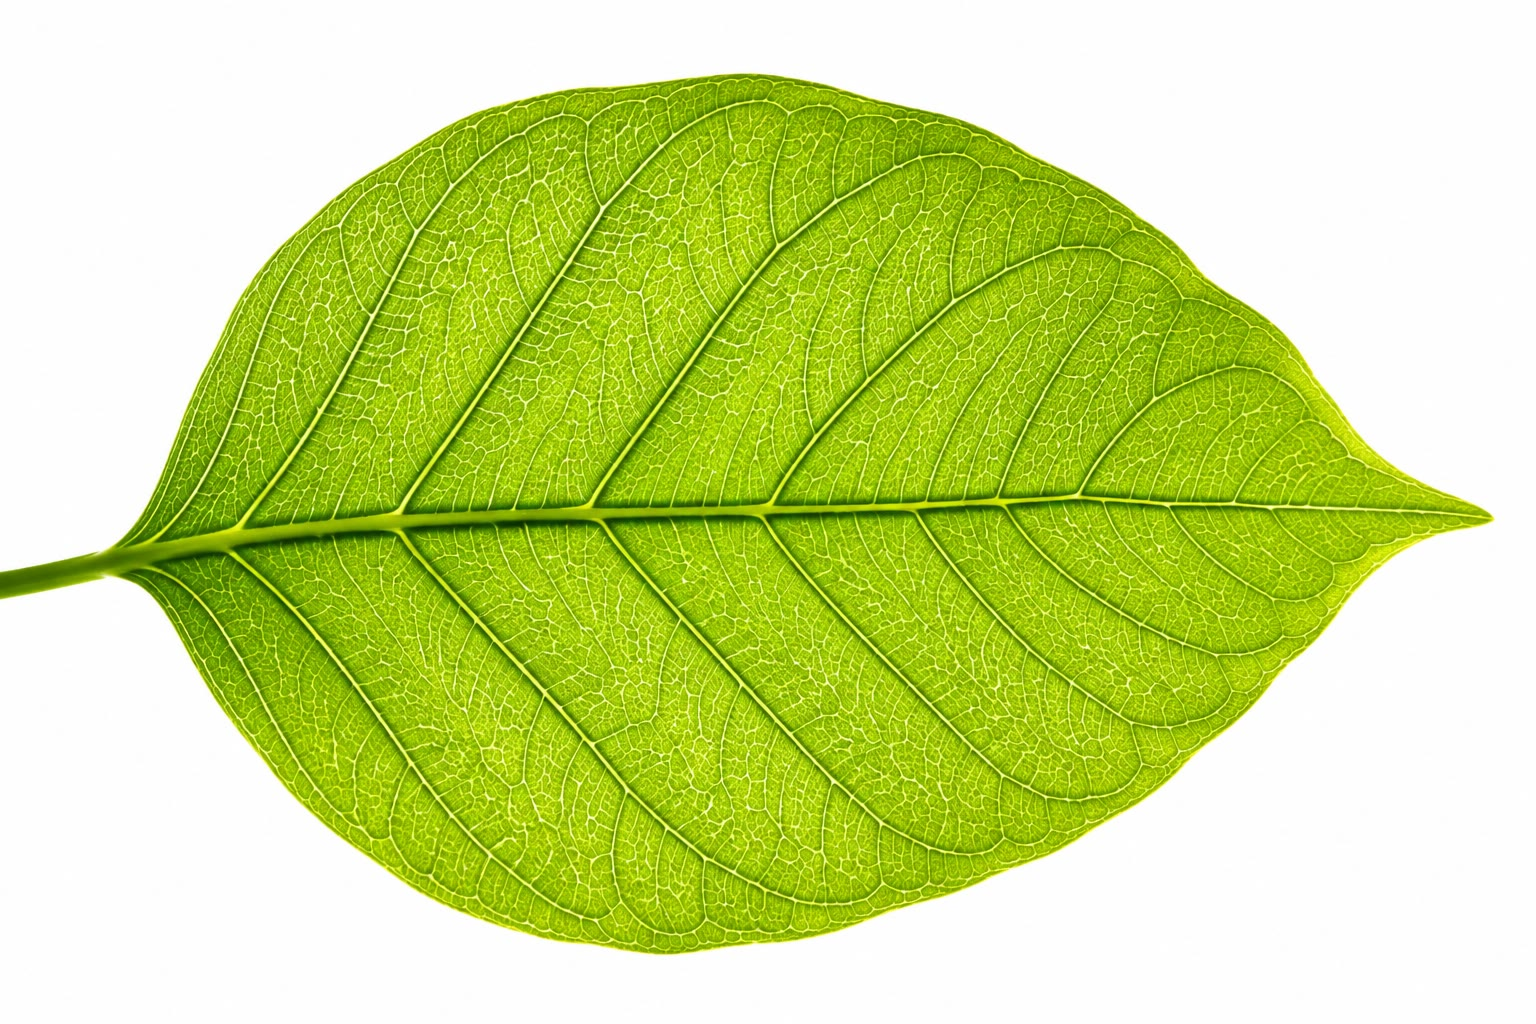
\includegraphics[width=0.6\linewidth]{images/book3/ai/b3-14-leaf-backlit.jpg}

{\small 迎着阳光的叶片：它吸收的光在栅栏\omterm{def:b1:cell-unit-of-life:cell}{细胞}
的每一个\omterm{def:b1:photosynthesis:chloroplast}{叶绿体}中驱动水的裂解和
二氧化碳的\omterm{def:b1:photosynthesis:fixation}{固定}，二氧化碳经由\omterm{def:b1:flowering-plant-organization:tissues}{气孔}进入叶片。}
\end{omfigure}

\begin{method}[光合作用收支核算]\label{met:b1:photosynthesis:budget}
\begin{enumerate}
  \item 计算碳数：每\omterm{def:b1:photosynthesis:fixation}{固定}一个 $\mathrm{CO_2}$，便得到一个碳的
        产物；一分子葡萄糖需要六轮 \omterm{def:b1:photosynthesis:fixation}{RuBisCO} 反应。
  \item 计算载体：每轮消耗 3 个 \omterm{def:b1:water-small-molecules:atp}{ATP} 和 2 个 NADPH（每个 G3P 为
        9 个 \omterm{def:b1:water-small-molecules:atp}{ATP} 和 6 个 NADPH）；一分子葡萄糖消耗 18 个 \omterm{def:b1:water-small-molecules:atp}{ATP} 和 12 个 NADPH。
  \item 计算光子：线性电子流给出 2 个 NADPH 和约 3 个 \omterm{def:b1:water-small-molecules:atp}{ATP}，
        每个 $\mathrm{O_2}$，对应 8 个光子（每个\omterm{def:b1:photosynthesis:zscheme}{光系统} 4 个）；12 个 NADPH
        需要 6 个 $\mathrm{O_2}$ 和 48 个光子；额外的 \omterm{def:b1:water-small-molecules:atp}{ATP} 来自
        环式电子流（再需少量光子）。每个
        $\mathrm{CO_2}$ 约需 8 个光子，即量子需求。
  \item 计算能量：一摩尔 \qty{680}{nm} 光子的能量为 \qty{176}{kJ}；
        48 个光子的能量为 \qty{8450}{kJ}，贮存于
        葡萄糖中的 \qty{2870}{kJ}，效率至多 \qty{34}{\%}，未计
        反射、呼吸作用及未被吸收的光谱部分的损失。
\end{enumerate}
\end{method}

\section{光呼吸、C4 与 CAM}

\begin{proposition}[RuBisCO 的缺陷]\label{prop:b1:photosynthesis:photorespiration}
\index{光呼吸}
\omterm{def:b1:photosynthesis:fixation}{RuBisCO} 也接受 $\mathrm{O_2}$ 代替 $\mathrm{CO_2}$：RuBP 的加氧反应
生成一分子 3-PGA 和一分子两碳的磷酸乙醇酸，
\omterm{def:b1:cell-unit-of-life:cell}{细胞}必须经由一条代价高昂、横跨三个
\omterm{def:b1:eukaryotic-cell:organelle}{细胞器}的途径加以挽救，该途径释放 $\mathrm{CO_2}$ 并消耗 \omterm{def:b1:water-small-molecules:atp}{ATP}——
\emph{光呼吸}。该酶的区分能力很差（浓度相等时，
约 \qty{80}{} 比 1 偏向 $\mathrm{CO_2}$），
而空气中 $\mathrm{O_2}$ 的丰度比
$\mathrm{CO_2}$ 高五百倍；在 \qty{25}{\celsius} 时，四分之一的\omterm{def:b1:photosynthesis:fixation}{固定}
被白白浪费，炎热干燥的天气里比例更高，此时\omterm{def:b1:flowering-plant-organization:tissues}{气孔}关闭，叶内
$\mathrm{CO_2}$ 浓度下降。\omterm{def:b1:photosynthesis:fixation}{RuBisCO} 进化于大气中没有氧气的时代，
也较慢（每秒三次周转），并以
丰度来补偿：它是地球上含量最丰富的\omterm{def:b1:proteins:peptide}{蛋白质}，占
叶片可溶性蛋白的一半。
\end{proposition}

\begin{definition}[C4 和 CAM 植物]\label{def:b1:photosynthesis:c4cam}
\index{C4 植物}\index{CAM 植物}
\emph{C4 植物}（玉米、甘蔗、高粱以及许多热带禾草）
通过浓缩 $\mathrm{CO_2}$ 堵住漏洞：在叶肉\omterm{def:b1:cell-unit-of-life:cell}{细胞}中，
一种对 $\mathrm{O_2}$ 没有亲和力的酶（PEP 羧化酶）将碳酸氢根
\omterm{def:b1:photosynthesis:fixation}{固定}为四碳酸，四碳酸被运入叶脉周围的
\emph{维管束鞘}\omterm{def:b1:cell-unit-of-life:cell}{细胞}，并在那里脱羧，
使 \omterm{def:b1:photosynthesis:fixation}{RuBisCO} 周围的 $\mathrm{CO_2}$ 浓度提高十倍，并抑制
加氧反应——代价是每\omterm{def:b1:photosynthesis:fixation}{固定}一个 $\mathrm{CO_2}$ 多消耗两个 \omterm{def:b1:water-small-molecules:atp}{ATP}。两类
\omterm{def:b1:cell-unit-of-life:cell}{细胞}共同构成\emph{花环}结构。\emph{CAM 植物}
（仙人掌、菠萝、龙舌兰）在时间而非空间上分离同样的两步：
它们夜间打开\omterm{def:b1:flowering-plant-organization:tissues}{气孔}，以苹果酸的形式将 $\mathrm{CO_2}$ 储存在
\omterm{def:b1:eukaryotic-cell:plantcell}{液泡}中，白天则在\omterm{def:b1:flowering-plant-organization:tissues}{气孔}关闭时将其释放给 \omterm{def:b1:photosynthesis:fixation}{RuBisCO}，
每\omterm{def:b1:photosynthesis:fixation}{固定}一个碳所失的水量，
仅为 C3 植物的十分之一。
\end{definition}

\begin{omfigure}
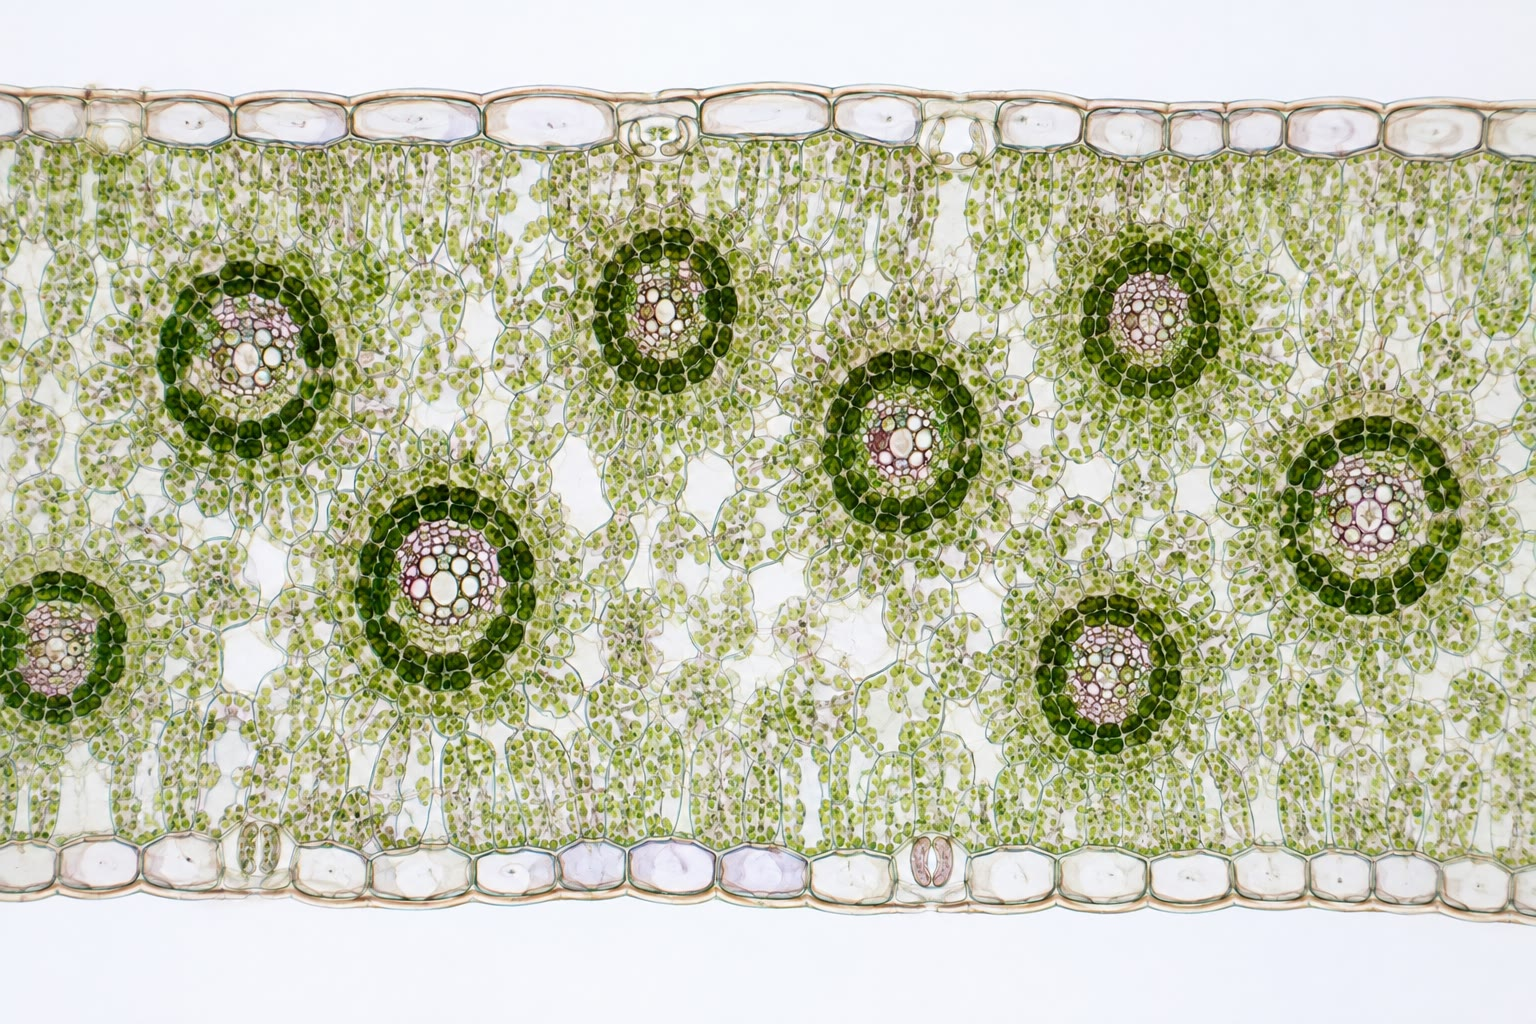
\includegraphics[width=0.6\linewidth]{images/book3/ai/b3-14-maize-kranz.jpg}

{\small 玉米叶片中的花环结构：每条叶脉被
大型维管束鞘\omterm{def:b1:cell-unit-of-life:cell}{细胞}环绕，这些\omterm{def:b1:cell-unit-of-life:cell}{细胞}内充满\omterm{def:b1:photosynthesis:chloroplast}{叶绿体}，
这些\omterm{def:b1:cell-unit-of-life:cell}{细胞}又被叶肉\omterm{def:b1:cell-unit-of-life:cell}{细胞}环绕。$\mathrm{CO_2}$ 在外环被捕获，
并被浓缩输送到内环的 \omterm{def:b1:photosynthesis:fixation}{RuBisCO}。}
\end{omfigure}

\begin{example}[哪种植物在哪里]\label{ex:b1:photosynthesis:where}
在 \qty{20}{\celsius}、潮湿空气中，C3 小麦叶片与 C4 玉米叶片
\omterm{def:b1:photosynthesis:fixation}{固定}碳的速率相近，但玉米每个碳要
多消耗两个 \omterm{def:b1:water-small-molecules:atp}{ATP}。在 \qty{35}{\celsius}、干燥空气中，小麦
因光呼吸损失三分之一的\omterm{def:b1:photosynthesis:fixation}{固定}量，玉米则毫无损失：C4 禾草
占据炎热开阔的地带，C3 植物则多见于凉爽和荫蔽处。仙人掌
无论采用哪种标准途径，\omterm{def:b1:photosynthesis:fixation}{固定}速度都很慢，但它能够
在其他植物都会渴死的地方存活。
\end{example}

\section{自养}

\begin{definition}[自养]\label{def:b1:photosynthesis:autotrophy}
\omterm{def:b1:organism-environment:organism}{生物体}以 $\mathrm{CO_2}$ 合成自身有机物时，称其为\emph{自养}\index{自养}的
（\cref{ch:b1:organism-environment}）。
它需要能量来源和电子来源。
\emph{\omterm{def:b1:organism-environment:trophy}{光能自养生物}}以光为能量来源：植物、藻类和
蓝细菌从水中获取电子并释放氧气
（\emph{产氧}）；紫色细菌和绿色细菌则从硫化氢
或有机酸中获取电子，且不释放氧气。\emph{\omterm{def:b1:organism-environment:trophy}{化能自养生物}}
同时从无机
化合物的氧化中获取能量和电子——氨、亚硝酸盐、硫化物、氢气、亚铁离子——完全
不需要光：土壤中的硝化细菌，以及
为深海热液喷口生态系统提供物质基础的细菌。所有自养生物都利用\omterm{def:b1:photosynthesis:fixation}{卡尔文循环}
或相关循环\omterm{def:b1:photosynthesis:fixation}{固定}碳；它们都以 NADPH 还原碳，并消耗 \omterm{def:b1:water-small-molecules:atp}{ATP}；
它们的区别仅在于 \omterm{def:b1:water-small-molecules:atp}{ATP} 和电子的
来源不同。
\end{definition}

\begin{example}[全球收支]\label{ex:b1:photosynthesis:global}
光合作用每年在陆地上\omterm{def:b1:photosynthesis:fixation}{固定}约 \qty{120}{Gt} 的碳，
在海洋中\omterm{def:b1:photosynthesis:fixation}{固定}约 \qty{50}{Gt}，其中一半由单\omterm{def:b1:cell-unit-of-life:cell}{细胞}藻类和
肉眼不可见的蓝细菌完成；它使大气中的二氧化碳
每七年完成一次更替，氧气每两千年完成一次更替。
氧气的来源也是如此：二十亿年来，蓝细菌
将氧气释放到原本没有氧气的大气中，而每一种需氧
\omterm{def:b1:organism-environment:organism}{生物体}，从\omterm{def:b1:eukaryotic-cell:mitochondrion}{线粒体}开始，都建立在某一种
分解水的酶系统所造成的泄漏之上。
\end{example}

\section{练习}

\begin{exercise}[$\star$]\label{exo:b1:photosynthesis:1}
说出\omterm{def:b1:photosynthesis:chloroplast}{叶绿体}的三类膜系统，并指出\omterm{prop:b1:photosynthesis:lightreactions}{光反应}与
\omterm{def:b1:photosynthesis:fixation}{卡尔文循环}分别在何处进行。
\end{exercise}

\begin{exercise}[$\star$]\label{exo:b1:photosynthesis:2}
写出\omterm{prop:b1:photosynthesis:lightreactions}{光反应}的方程式，并说明释放的
氧气来自何处，并给出证据。
\end{exercise}

\begin{exercise}[$\star$]\label{exo:b1:photosynthesis:3}
说出\omterm{def:b1:photosynthesis:fixation}{卡尔文循环}的三个阶段，以及每\omterm{def:b1:photosynthesis:fixation}{固定}一个
$\mathrm{CO_2}$ 所消耗的 \omterm{def:b1:water-small-molecules:atp}{ATP} 和 NADPH 数量。
\end{exercise}

\begin{exercise}[$\star$]\label{exo:b1:photosynthesis:4}
根据光谱图，\omterm{def:b1:photosynthesis:pigments}{叶绿素} $a$ 在哪些波长处
吸收最多？为什么作用光谱
在 \qty{500}{nm} 附近高于\omterm{def:b1:photosynthesis:pigments}{叶绿素}的吸收？
\end{exercise}

\begin{exercise}[$\star\star$]\label{exo:b1:photosynthesis:5}
解释爱默生增益效应，以及它揭示了\omterm{prop:b1:photosynthesis:lightreactions}{光反应}的
何种\omterm{def:b1:body-plans-tissues:tissue}{组织}方式。
\end{exercise}

\begin{exercise}[$\star\star$]\label{exo:b1:photosynthesis:6}
质子动力势为 \qty{0.18}{V} 时，每摩尔质子对应
多少\omterm{prop:b1:water-small-molecules:gibbs}{自由能}（$F = \qty{96500}{C/mol}$）？
在 \qty{50}{kJ/mol} 下合成一个 \omterm{def:b1:water-small-molecules:atp}{ATP} 需要多少质子流过？与
合酶所用的四个质子相比如何？
\end{exercise}

\begin{exercise}[$\star\star$]\label{exo:b1:photosynthesis:7}
雅根多夫的\omterm{def:b1:photosynthesis:chloroplast}{类囊体}在酸浴后，于黑暗中
合成了 \omterm{def:b1:water-small-molecules:atp}{ATP}。解释这一实验证明了什么、没有证明什么，
并预测若在质子转移前加入解偶联剂，结果如何。
\end{exercise}

\begin{exercise}[$\star\star$]\label{exo:b1:photosynthesis:8}
追踪碳的去向：从 3 个 RuBP（15 个碳）和 3
个 $\mathrm{CO_2}$ 出发，依次计算 3-PGA、G3P、输出的 G3P 和
再生的 RuBP 中的碳数，并验证其平衡。
\end{exercise}

\begin{exercise}[$\star\star$]\label{exo:b1:photosynthesis:9}
在卡尔文实验中，去除 $\mathrm{CO_2}$ 时 RuBP 上升、3-PGA 下降；
关闭光照时 3-PGA 上升、RuBP 下降。
从循环角度解释这两种变化。
\end{exercise}

\begin{exercise}[$\star\star\star$]\label{exo:b1:photosynthesis:10}
计算一摩尔 \qty{680}{nm} 光子的能量（$h =
\qty{6.63e-34}{J.s}$, $c = \qty{3.0e8}{m/s}$, $N_A = \num{6.02e23}$),
每个葡萄糖所需 48 个光子的能量，以及
储存 \qty{2870}{kJ/mol} 的效率；为什么整株作物的效率
仅约为日光的 \qty{1}{\%}，要低得多？
\end{exercise}

\begin{exercise}[$\star\star\star$]\label{exo:b1:photosynthesis:11}
在 \qty{25}{\celsius} 的空气中，\omterm{def:b1:photosynthesis:fixation}{RuBisCO} 每进行三次羧化
便发生一次加氧；每次加氧经回收释放半个 $\mathrm{CO_2}$，
回收过程还需消耗 \omterm{def:b1:water-small-molecules:atp}{ATP}。计算每 100 次羧化净\omterm{def:b1:photosynthesis:fixation}{固定}的碳量
及损失的比例。C4 植物可避免该损失，但
每\omterm{def:b1:photosynthesis:fixation}{固定}一个 $\mathrm{CO_2}$ 多耗 2 个 \omterm{def:b1:water-small-molecules:atp}{ATP}，损失比例为多少时
C4 设计何时划算？假设一个 \omterm{def:b1:water-small-molecules:atp}{ATP} 约值 $\mathrm{CO_2}$
\omterm{def:b1:photosynthesis:fixation}{固定}量的十分之一。
\end{exercise}

\begin{exercise}[$\star\star\star$]\label{exo:b1:photosynthesis:12}
“光合作用是逆向运行的呼吸作用。”请用一段文字讨论，
比较化学渗透机制、电子流动的方向、
载体与循环，并指出这一类比在何处成立、
在何处失效。
\end{exercise}

\section{问题：一个葡萄糖分子的代价}

\begin{problem}[{周末问题——清点光子，追踪电子与质子穿过类囊体，
核算并消耗 ATP 与 NADPH，
称量一片叶子的日产量，最后落到
光合作用的能量效率上}]
\label{pb:b1:photosynthesis:1}
常数：$h = \qty{6.63e-34}{J.s}$，$c = \qty{3.00e8}{m/s}$，
$N_A = \num{6.02e23}$, $F = \qty{96500}{C/mol}$, $R = \qty{8.314}{J.mol^{-1}.K^{-1}}$,
$T = \qty{298}{K}$。葡萄糖燃烧的\omterm{prop:b1:water-small-molecules:gibbs}{自由能}
为 \qty{2870}{kJ/mol}；\omterm{def:b1:photosynthesis:chloroplast}{叶绿体}中合成 \omterm{def:b1:water-small-molecules:atp}{ATP} 的代价为
\qty{50}{kJ/mol}；NADPH 含有 \qty{220}{kJ/mol} 的还原力。

\medskip
\noindent\textbf{第一部分——光子与电子。}
\begin{enumerate}
  \item 计算一个 \qty{680}{nm} 光子的能量，以及
        一摩尔这种光子的能量。
  \item 计算一摩尔 \qty{700}{nm} 光子与
        \qty{450}{nm} 光子的能量。为何蓝光每个光子的
        光合作用效果不超过红光？
  \item 一焦耳的 \qty{680}{nm} 光子有多少个？
  \item 将一个电子从水（$E'_0 = \qty{+0.82}{V}$）转移到
        $\mathrm{NADP^+}$（$E'_0 = \qty{-0.32}{V}$）需要多少
        每摩尔电子的\omterm{prop:b1:water-small-molecules:gibbs}{自由能}（$\Delta G = -nF\Delta E$）？
  \item 每个电子需用两个光子（每个\omterm{def:b1:photosynthesis:zscheme}{光系统}各一个）。
        计算每摩尔电子所获得的能量，以及
        其中储存于氧化还原变化中的比例。
  \item 需要多少个电子（进而多少个光子）才能制得
        一个 $\mathrm{O_2}$ 和两个 NADPH？
  \item 若需 12 个 NADPH，每个葡萄糖需要多少个光子？
\end{enumerate}

\medskip
\noindent\textbf{第二部分——质子与 \omterm{def:b1:water-small-molecules:atp}{ATP}。}
每释放一个 $\mathrm{O_2}$，水裂解在\omterm{def:b1:photosynthesis:chloroplast}{类囊体}腔中释放四个质子，
另有八个质子被\omterm{def:b1:cell-unit-of-life:cell}{细胞}色素 $b_6f$
复合体泵入\omterm{def:b1:photosynthesis:chloroplast}{类囊体}腔；\omterm{def:b1:water-small-molecules:atp}{ATP} 合酶每个 \omterm{def:b1:water-small-molecules:atp}{ATP} 需 \qty{4}{H^+}。\omterm{def:b1:photosynthesis:chloroplast}{类囊体}腔的
\omterm{def:b1:water-small-molecules:ph}{pH} 为 5，\omterm{def:b1:photosynthesis:chloroplast}{基质}的 \omterm{def:b1:water-small-molecules:ph}{pH} 为 8；跨\omterm{def:b1:photosynthesis:chloroplast}{类囊体}膜的\omterm{def:b1:membranes-transport:potential}{膜电位}
可忽略不计。
\begin{enumerate}[resume]
  \item 由 \omterm{def:b1:water-small-molecules:ph}{pH} 差计算质子动力势（以伏特计）
        （$\Delta\mu = 2.303\,RT\,\Delta\mathrm{pH}/F$），以及
        每摩尔质子的\omterm{prop:b1:water-small-molecules:gibbs}{自由能}。
  \item 计算每个 $\mathrm{O_2}$ 向\omterm{def:b1:photosynthesis:chloroplast}{类囊体}腔输送的质子数，
        以及它们可合成的 \omterm{def:b1:water-small-molecules:atp}{ATP} 数。
  \item 按线性电子流计算每个葡萄糖产生的 \omterm{def:b1:water-small-molecules:atp}{ATP} 数（释放 6
        个 $\mathrm{O_2}$），并与\omterm{def:b1:photosynthesis:fixation}{卡尔文循环}所需的
        18 个相比较，该缺口如何补足？
  \item 计算每个 \omterm{def:b1:water-small-molecules:atp}{ATP} 可获得的质子\omterm{prop:b1:water-small-molecules:gibbs}{自由能}，
        （\qty{4}{H^+}）以及 \omterm{def:b1:water-small-molecules:atp}{ATP} 合酶的效率。
  \item \omterm{def:b1:photosynthesis:chloroplast}{叶绿体}的\omterm{def:b1:photosynthesis:chloroplast}{类囊体}腔体积约为
        \qty{1}{\micro m^3}。\omterm{def:b1:water-small-molecules:ph}{pH} 为 5 时，其中含有多少游离质子？
        与每秒经合酶通过的约 $10^5$ 个质子相比，
        并推断什么物质在缓冲
        \omterm{def:b1:photosynthesis:chloroplast}{类囊体}腔。
\end{enumerate}

\medskip
\noindent\textbf{第三部分——糖。}
\begin{enumerate}[resume]
  \item 将每个葡萄糖储存的能量写作 18 个 \omterm{def:b1:water-small-molecules:atp}{ATP} $\times$
        \qty{50}{kJ} 加 12 个 NADPH $\times$ \qty{220}{kJ}，并与
        葡萄糖的 \qty{2870}{kJ} 相比较，其差额
        去向何处？
  \item 计算第 6 小题中 48 个光子的能量，以及
        从光子到葡萄糖的光合作用效率。
  \item 日光中只有 \qty{45}{\%} 处于色素所吸收的波段，
        其中十分之一被反射或透过，
        计算从入射日光到葡萄糖的效率，
        尚未扣除呼吸作用。
  \item 一片面积为 \qty{50}{cm^2} 的叶片接收 \qty{400}{W/m^2} 的日光
        照射 \qty{10}{h}。计算所接收的能量，并按
        第 14 小题的效率，计算所制葡萄糖的质量，以克计，
        摩尔质量取 \qty{180}{g/mol}。
  \item 叶片将其中 \qty{40}{\%} 的葡萄糖用于呼吸作用以维持生命。
        其净增益为多少，以葡萄糖的克数和
        碳的克数分别表示？
  \item 一季作物的总效率达到 \qty{1}{\%}。列出
        除上述已计入的损失外，列出三种损失，它们使叶片的
        数值与作物的数值有所区别。
\end{enumerate}

\medskip
\noindent\textbf{第四部分——漏损。}
在 \qty{25}{\celsius} 的空气中，\omterm{def:b1:photosynthesis:fixation}{RuBisCO} 每进行三次羧化
便发生一次加氧；每次加氧相当于损失半个
$\mathrm{CO_2}$ \omterm{def:b1:photosynthesis:fixation}{固定}量的一半，并耗 3.5 个 \omterm{def:b1:water-small-molecules:atp}{ATP}。
\begin{enumerate}[resume]
  \item 计算每 100 次羧化中的加氧次数、碳损失量
        及净碳得量。
  \item 计算每 100 次羧化用于回收的 \omterm{def:b1:water-small-molecules:atp}{ATP}，以及
        每获得单位净碳所需的总 \omterm{def:b1:water-small-molecules:atp}{ATP}（\omterm{def:b1:photosynthesis:fixation}{卡尔文循环}每次羧化耗 3 个 \omterm{def:b1:water-small-molecules:atp}{ATP}，
        另加回收所耗的 \omterm{def:b1:water-small-molecules:atp}{ATP}）。
  \item C4 植物没有加氧反应，但每输送一个
        $\mathrm{CO_2}$ 需多耗 2 个 \omterm{def:b1:water-small-molecules:atp}{ATP}。计算其每单位净碳所耗 \omterm{def:b1:water-small-molecules:atp}{ATP}，并
        加以比较。
  \item 在 \qty{35}{\celsius} 时，加氧与羧化之比升至一比二，
        重新计算 C3 的数值，并说明哪种设计更优。
  \item 解释为何将温室中的 $\mathrm{CO_2}$ 浓度提高到
        大气值的三倍，会提高 C3 作物（番茄、小麦）的产量，
        却几乎不影响 C4 作物（玉米）的产量。
  \item 每\omterm{def:b1:photosynthesis:fixation}{固定}一个 $\mathrm{CO_2}$，C3 叶片约失去 250 个水分子，
        而 CAM 植物\omterm{def:b1:photosynthesis:fixation}{固定}时约为 25 个。计算两者为\omterm{def:b1:photosynthesis:fixation}{固定}
        \qty{1}{g} 碳所失去的水量。
  \item 给出结果：每个 $\mathrm{CO_2}$ 的量子需求、
        从光子到葡萄糖的效率，以及从
        日光到叶片净产糖的效率。
\end{enumerate}
\end{problem}
